% Template article for preprint document class `elsart'
% with harvard style bibliographic references
% SP 2001/01/05

%\documentclass[doublespacing]{elsart}
%\documentclass[reviewcopy]{elsart}
\documentclass{elsart}
\journal{Expert Systems with Applications}
%\usepackage{epsf}
\usepackage{algorithm,algorithmic}
\usepackage[dvips]{graphicx}
\usepackage{amssymb, amsmath}
\usepackage{ascmac}
\usepackage{cite}
%\usepackage{url}
\usepackage{amsmath}
%\usepackage{amssymb}
\usepackage{booktabs}
%\usepackage{latexsym}
%\usepackage{array}
%\usepackage{enumerate}
\usepackage{multirow}
\usepackage{apacite}



\usepackage{epsfig}
\usepackage[caption=false]{subfig}
\usepackage{latexsym}
\usepackage{ascmac}

\usepackage{amssymb, amsmath}
\usepackage{array}
% Use the option doublespacing or reviewcopy to obtain double line spacing
% \documentclass[doublespacing]{elsart}
%\usepackage{epsf}


% if you use PostScript figures in your article
% use the graphics package for simple commands
% \usepackage{graphics}
% or use the graphicx package for more complicated commands
%\usepackage[dvips]{graphicx}
% or use the epsfig package if you prefer to use the old commands
%% \usepackage{epsfig}


% The amssymb package provides various useful mathematical symbols
\usepackage{amssymb}

% the natbib package allows both number and author-year (Harvard)
% style referencing;
%\usepackage[authoryear]{natbib}
%\usepackage{natbib}

\begin{document}

\begin{frontmatter}

% Title, authors and addresses

% use the thanksref command within \title, \author or \address for footnotes;
% use the corauthref command within \author for corresponding author footnotes;
% use the ead command for the email address,
% and the form \ead[url] for the home page:
% \title{Title\thanksref{label1}}
% \thanks[label1]{}
% \author{Name\corauthref{cor1}\thanksref{label2}}
% \ead{email address}
% \ead[url]{home page}
% \thanks[label2]{}
% \corauth[cor1]{}
% \address{Address\thanksref{label3}}
% \thanks[label3]{}

\title{Combination of Genetic Network Programming and Knapsack Problem to Support Record Clustering on Distributed Databases}

% use optional labels to link authors explicitly to addresses:
% \author[label1,label2]{}
% \address[label1]{}
% \address[label2]{}

\author[label1]{Wirarama Wedashwara}\ead{t001we@yamaguchi-u.ac.jp},
\author[label1]{Shingo Mabu\corauthref{cor1}}\ead{mabu@yamaguchi-u.ac.jp},
\author[label1]{Masanao Obayashi}\ead{m.obayas@yamaguchi-u.ac.jp},
\author[label1]{Takashi Kuremoto}\ead{wu@yamaguchi-u.ac.jp}

\corauth[cor1]{Corresponding author. Tel.: +81-836-85-9519; Fax.: +81-836-85-9519}
\address[label1]{Graduate School of Science and Engineering, Yamaguchi University, Tokiwadai 2-16-1, Ube, Yamaguchi, 755-8611,  Japan}

\begin{abstract}
This research involves implementation of genetic network programming (GNP) and knapsack problem (KP) as a decision support system for record clustering in distributed databases. The objective is to distribute big data to certain sites with the limited amount of capacities by considering the similarity of distributed data in each site. GNP is used to extract rules from big data by considering characteristics (value ranges) of each attribute in a dataset. KP is used to distribute rules to each site by considering similarity (value) and data amount (weight) related to each rule to match the site capacities. From the simulation results, it is clarified that the proposed method shows some advantages over the conventional clustering algorithms. 
\end{abstract}


\begin{keyword}
% keywords here, in the form: keyword \sep keyword
Genetic Network Programming
\sep Database Clustering
\sep Knapsack Problem
\sep Record Clustering
% PACS codes here, in the form: \PACS code \sep code
\end{keyword}
\end{frontmatter}

% main text

\section{Introduction}

\begin{figure}[tb]
\begin{center}
\includegraphics[width=8cm]{images/ddbms}
\caption{\label{ddbms} A distributed database environment}
\end{center}
\end{figure}

Distributed database management system (DDBMS) could be a solution for large scale information systems with large amount of data growth and data accesses. A distributed database (DDB) is a collection of data that logically belongs to the same system but is spread over the sites of a computer network (Fig. \ref{ddbms}). A DDBMS is then defined as a software system that permits the management of DDB and makes the distribution of data between databases and software transparent to the users \cite{horizontalfragmentation,horizontalfragmentation1}.

To handle the data proliferation, efficient access methods and data storage techniques have become increasingly critical to maintain an acceptable query response time. One way to improve query response time is to reduce the number of disk I/Os by clustering the database vertically (attribute clustering) and/or horizontally (record clustering) \cite{recordclustering,recordclustering1}. Improvements in the retrieval time of multi-attribute records can be attained if similar records are grouped close together in the file space as a result of restructuring. This is because fewer page transfers are required as the probability of two or more of the target records residing in the same page of storage is increased \cite{recordclustering2}.

In this paper, a novel method combining genetic network programming (GNP) \cite{gnp1,gnp2} and knapsack problem (KP) \cite{knapsack2,knapsack3} for record clustering is proposed. Hypothesis of this research are the implementation of GNP for data mining can create effective clusters from complicated datasets and KP can handle the problem of distributing fragments to several sites considering value (similarity of data) and mass (data size) in DDBMS. Therefore, it could be a solution to the fragment allocation and site storage capacity problems.

This paper is organized as follows. Section 2 describes a review of the proposed framework, section 3 describes the detailed algorithm of the proposed framework, section 4 shows the simulation results, and finally section 5 is devoted to conclusions.

%%% Section 2 %%%%%%%%%%%%%%%%%%%%%%%%%%%%%%%%%%%%%%%%
\section{Review of the Proposed Framework}

\subsection{Genetic Network Programming}

\begin{figure}[tb]
\begin{center}
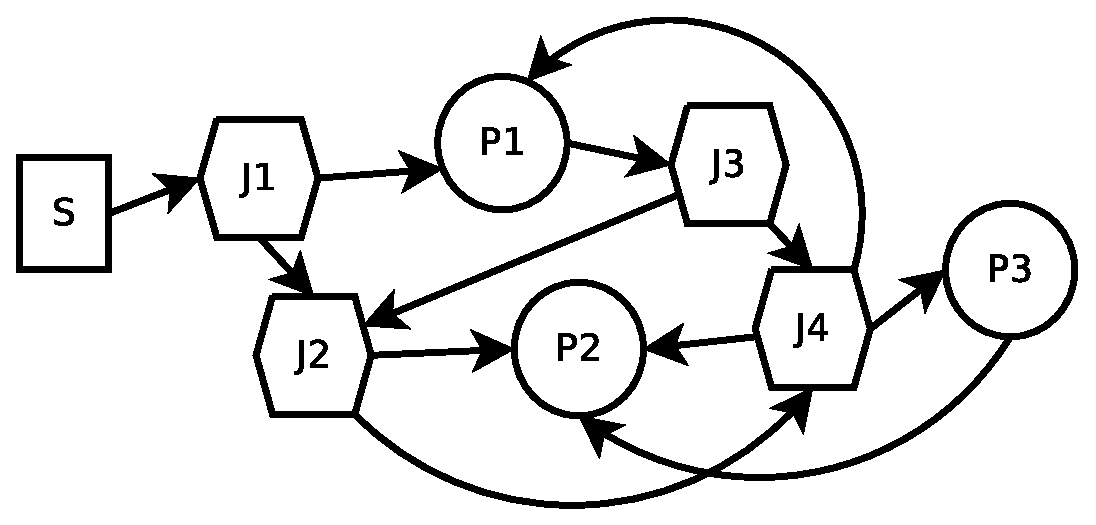
\includegraphics[width=8cm]{images/gnpbasic}
\caption{\label{gnpbasic} Basic Implementation of GNP}
\end{center}
S : start node, [$J_{1}$,...,$J_{4}$] : judgement node, [$P_{1}$,...,$P_{3}$] : processing node
\end{figure}

GNP is an evolutionary optimization technique, which uses directed graph structures instead of strings in genetic algorithm \cite{holland1975} or trees in genetic programming \cite{koza1992}, which leads to enhancing the representation ability with compact programs derived from the re-usability of nodes in a graph structure.

In GNP, nodes are interpreted as the minimum units of judgement and action, and node transition represents rules of the program. After starting the node transition from the start node, GNP does not return to the start node when the actions are completed. The next judgement and action are always influenced by the previous node transition. Judgement and processing of GNP programs are performed on the node level.

The basic structure of GNP is illustrated in Fig. \ref{gnpbasic}, with $S$ denoting the start node. Two other kinds of nodes, judgement nodes and processing nodes, have judgement function $J_{p}$ and processing function $P_{q}$, respectively. $J_{p}$ ($p = 1,\dots, n$) denotes the $p$-th judgement function stored in a library for judgement nodes, while $P_{q}$ ($q = 1,\dots, m$) denotes the $q$-th processing function stored in a library for processing nodes \cite{gnp1, gnp2}.

In this research, GNP is used to handle rule extraction from datasets by analyzing the records. Each judgment node represents an attribute with value range. For example, price attribute could be divided into three ranges (low, middle, high), and one range is assigned to one judgment node. GNP makes rules by evolving combinations of nodes and measures the coverage of the extracted rules. Coverage means that how much records in a dataset each rule can represent (cover). Rules that cover at least one record will be stored in the rule pool, then in the KP phase, the stored rules are distributed to several sites. The point of this paper is to distribute rules, not the data, which contributes to distributing any data into the sites considering the similarities between rules and data. The detailed explanation of the implementation of GNP in rule extraction is available in section 3.1.

\subsection{Knapsack Problem}
KP is a combinational optimization problem dealing with a set of items, each with a mass and a value, determining the number of each item to include in a collection so that the total weight is less than or equal to the given limit and the total value is as large as possible. KP is defined as follows.

\begin{eqnarray}
\begin{array}{lll}
\text{maximize}~S=\underset{i=1}{\overset{n}{\sum}}v_{i}x_{i}, \text{~~subject to~~~} \underset{i=1}{\overset{n}{\sum}}w_{i}x_{i}\leq W,
\end{array}
\label{eq:knapsack-problem}
\end{eqnarray}

where $S=$ total value of the knapsack (site); $i$ = fragment number ($1 \leq i \leq n$); $x_{i}$ = the number of fragments $i$; $v_{i}$ = value (similarity to the leader rule of the site) of fragment $i$; $w_{i}$ = weight (data size) of fragment $i$; $W$ = capacity of the site.
By allowing each fragment (item) to be added more than once to sites, this optimization can handle the problem of replication \cite{knapsack, knapsack2}. 

Knapsack problem in this research is solved by standard dynamic programming for 0/1 knapsack problem \cite{knapsack_DP}.
Let us define two dimensional array $m[i,w]$ with row $i$ and column $w$.
$m[i,w]$ shows the value of knapsack when considering items with item number $1,2,\dots,i-1,i$, and their total weight $w$. 
$m[i,w]$ is calculated by Eq. \ref{eq:knapsack-problem1}.

\begin{eqnarray}
\begin{array}{lll}
    m[i,\,w]=m[i-1,\,w] \text{~~if~~} w_i > W\,\! \\
    m[i,\,w]=\max(m[i-1,\,w],\,m[i-1,w-w_i]+v_i) \text{~~if~~} w_i \leqslant W.
\end{array}
\label{eq:knapsack-problem1}
\end{eqnarray}

The first step is to calculate $m[0,w]$, then $m[1,w]$ is calculated based on the values of $m[0,w]$.
The same process is repeated to calculate $m[2,w], \dots, m[n,w]$.
After finishing calculating $m[i,w]$, the maximum value among all $m[n,w]$ $(0 \leq w \leq W)$ is selected as a solution of the problem.

In this research, KP is used to handle a distribution of rules extracted by GNP to each site. Rules with high data coverage will be the leaders of each site and KP will consider the similarity between the leader rules and remaining rules (which is considered as a value of item (rule) in KP) and coverage of rules (which is considered as weight in KP) should be matched with site capacities. Therefore, the similar rules to a certain leader are basically put into the same site.
Detailed explanation of the implementation of KP in the rule distribution is available in section 3.2.


\section{Combination of GNP and Knapsack problem}

Implementation for processing record clustering is separated into two parts: GNP rule extraction and KP rule distribution.

\subsection{GNP Rule Extraction\label{sec:gnp-rule-extraction}}

GNP is used to extract rules from a database by analyzing the database structure including:
\begin{description}
\item [Attributes amount]: the number of attributes in a dataset. Each attribute will be divided into some nodes depending on its variation and value ranges (distance of minimum value and maximum value). 
\item [Data amount]: the number of records in a dataset.
\item [Data variation]: how much different records are contained in a dataset. If every record in a dataset is different, variation is 100\%, if half of the records in the dataset is different, variation is 50\%, and if every record in a dataset is the same, variation is $1/$(the number of data)$ \times 100\%$. For example, in Table \ref{frequency-table} that will be shown in the later page, there are six data variation in total 310 data, so the variation is $(6/300)\times100=1.94\%$.
\end{description}

GNP is used to extract rules from a dataset by analyzing all the records. Phenotype and genotype structures of GNP are described in Fig. \ref{gnpdatamining} and Table \ref{gnp-gene-structure}, respectively. In Fig. \ref{gnpdatamining}, each node has its own node number (1--11), and in Table \ref{gnp-gene-structure}, the node information of each node number is described. The program size depends on the number of nodes, which affects the amount of rules created by the program. 

\begin{figure}[tb]
\begin{center}
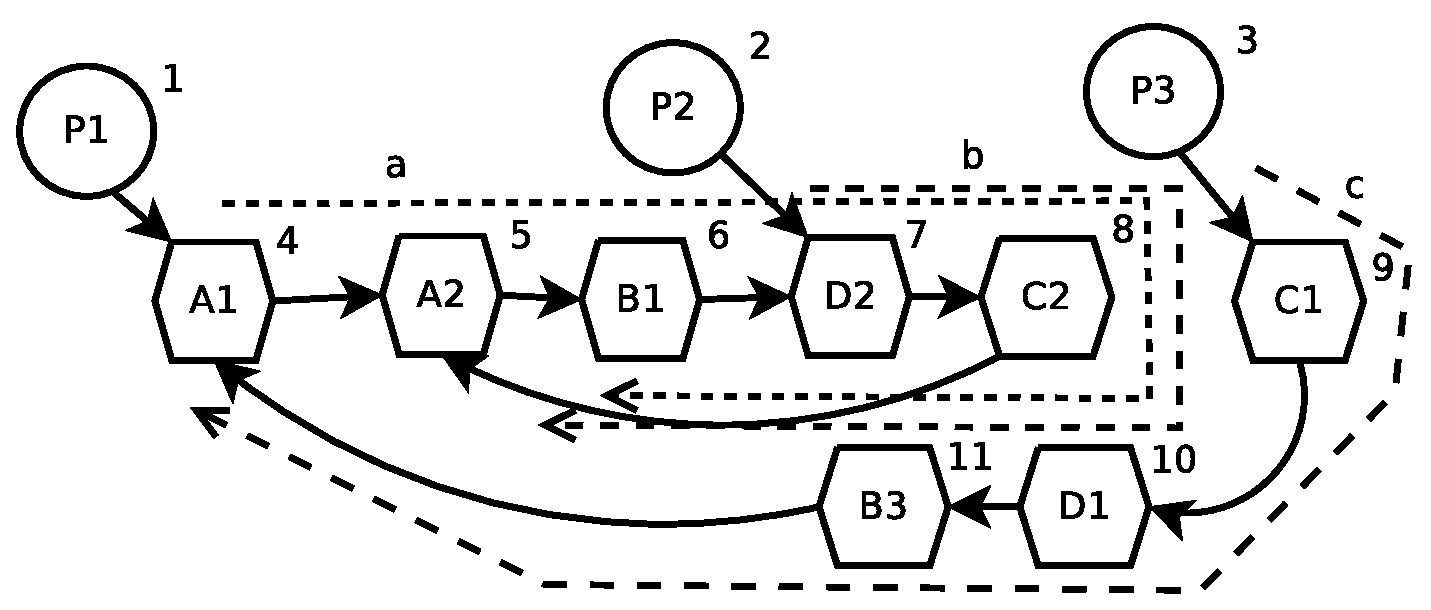
\includegraphics[width=10cm]{images/gnpdatamining}
\caption{\label{gnpdatamining} GNP Implementation on Data Mining}
\end{center}
\end{figure}

\begin{table}[tb]
\begin{minipage}[b]{0.4\linewidth}\centering
\caption{\label{gnp-gene-structure}GNP gene structure of Fig. \ref{gnpdatamining}}
\begin{flushleft}
\begin{tabular}{|c|c|c|c|c|}
\hline 
$i$ & $NT_{i}$ & $A_{i}$ & $R_{i}$ & $C_{i}$\tabularnewline
\hline 
1 & 1 & 0 & 0 & 4\tabularnewline
\hline 
2 & 1 & 0 & 0 & 7\tabularnewline
\hline 
3 & 1 & 0 & 0 & 9\tabularnewline
\hline 
4 & 2 & A & 1 & 5\tabularnewline
\hline 
5 & 2 & A & 2 & 6\tabularnewline
\hline 
6 & 2 & B & 1 & 7\tabularnewline
\hline 
7 & 2 & D & 2 & 8\tabularnewline
\hline 
8 & 2 & C & 2 & 5\tabularnewline
\hline 
9 & 2 & C & 1 & 10\tabularnewline
\hline 
10 & 2 & D & 1 & 11\tabularnewline
\hline 
11 & 2 & B & 3 & 4\tabularnewline
\hline 
\end{tabular}
\end{flushleft}
\end{minipage}
\begin{minipage}[b]{0.6\linewidth}
\begin{description}
\item [$i$] : Node number, 
\item [$NT_{i}$] : Node types; 1=processing, 2=judgment, 
\item [$A_{i}$] : Attribute index, 
\item [$R_{i}$] : Attribute range index, 
\item [$C_{i}$] : Connection
\end{description}
\end{minipage}
\end{table}


In the implementation of data mining, judgment node represents an attribute of the dataset, which is represented by $A_{i}$ showing an attribute index such as price, stock, etc., and $R_{i}$ showing a range index of an attribute value. For example, $A_{i}=A$ represents price attribute, and $R_{i}=1$ represents value range $[0,50]$ and $R_{i}=2$ represents value range $[51,80]$. Processing nodes show the start point of the sequence of judgment nodes which are executed sequentially by their connection. Sequences of nodes starting from each processing node $(P_{1},P_{2},P_{3})$ are represented by dotted line $a$, $b$ and $c$. A node sequence flows until support for the next combination does not satisfy the threshold. The nodes with the attributes that have already appeared in the sequence will be skipped. Candidate rules extracted by the program of Fig. \ref{gnpdatamining} to the dataset of Table \ref{dataset-support1} are shown in Table \ref{dataset-support2}. In Table \ref{dataset-support2}, three rules are extracted by the node sequence from each processing node. %but in other cases, node sequences can extract any number of rules depending on the connections %of judgment nodes. 

The score of rule is defined as follows.

\begin{eqnarray}
\begin{array}{lll}
\text{Score of rule \it{r}}=\begin{cases} 0 \;\text{if}\; sup(r)=0 & \\ 10*sup(r)+10*(n_{con}(r)-1) \;\text{if}\; sup(r)>0, \end{cases}
\end{array}
\label{eq:fitness}
\end{eqnarray}

where $sup(r)$ is the support\footnote{Ratio of records that satisfy rule $r$} of rule $r$ and $n_{con}(r)$ is the length of rule $r$.

Fitness for evaluating an individual is defined as follows.

\begin{eqnarray}
\begin{array}{lll}
\text{Fitness}=\underset{r\in R}{\sum}\{sup(r)+10(n_{con}(r)-1)+\alpha_{new}(r)\},
\end{array}
\label{eq:fitness1}
\end{eqnarray}
where $\alpha_{new}(r)$ is an additional value if rule $r$ is newly extracted.

\begin{table}[tb]
\caption{\label{dataset-support1}Example of dataset}
\begin{flushleft}
\begin{tabular}{|c|c|c|c|c|c|c|c|}
\hline 
$A_{1}$ & $A_{2}$ & $B_{1}$ & $D_{2}$ & $C_{2}$ & $C_{1}$ & $D_{1}$ & $B_{3}$\tabularnewline
\hline 
1 & 0 & 1 & 0 & 0 & 1 & 1 & 0\tabularnewline
\hline 
1 & 0 & 1 & 1 & 1 & 0 & 0 & 0\tabularnewline
\hline 
0 & 1 & 0 & 1 & 1 & 0 & 0 & 0\tabularnewline
\hline 
0 & 1 & 0 & 1 & 0 & 1 & 0 & 1\tabularnewline
\hline 
1 & 0 & 1 & 0 & 1 & 0 & 1 & 0\tabularnewline
\hline 
1 & 0 & 0 & 0 & 0 & 1 & 1 & 1\tabularnewline
\hline 
\end{tabular}
\end{flushleft}
\end{table}

\begin{table}[tb]
\caption{\label{dataset-support2}Example of dataset and its support to the extracted rules}
\begin{flushleft}
\begin{tabular}{|c|c|c|c|c|}
\hline 
\multirow{2}{*}{Processing Nodes} & \multirow{2}{*}{Extracted Rules} & \multirow{2}{*}{Support} & \multicolumn{2}{c|}{Score}\tabularnewline
\cline{4-5} 
 &  &  & Rule & Template\tabularnewline
\hline 
\multirow{3}{*}{1} & $A_{1}\wedge B_{1}$ & 3/6 & 15.00 & 6.00\tabularnewline
\cline{2-5} 
 & $A_{1}\wedge B_{1}\wedge D_{2}$ & 1/6 & 21.66 & 3.67\tabularnewline
\cline{2-5} 
 & $A_{1}\wedge B_{1}\wedge D_{2}\wedge C_{2}$ & 1/6 & 31.66 & 4.67\tabularnewline
\hline 
\multirow{3}{*}{2} & $D_{2}\wedge C_{2}$ & 2/6 & 11.66 & 4.33\tabularnewline
\cline{2-5} 
 & $D_{2}\wedge C_{2}\wedge A_{2}$ & 1/6 & 21.66 & 3.67\tabularnewline
\cline{2-5} 
 & $D_{2}\wedge C_{2}\wedge A_{2}\wedge B_{1}$ & 0/6 & 0 & 0\tabularnewline
\hline 
\multirow{3}{*}{3} & $C_{1}\wedge D_{1}$ & 2/6 & 13.33 & 4.33\tabularnewline
\cline{2-5} 
 & $C_{1}\wedge D_{1}\wedge B_{3}$ & 1/6 & 21.66 & 3.67\tabularnewline
\cline{2-5} 
 & $C_{1}\wedge D_{1}\wedge B_{3}\wedge A_{1}$ & 1/6 & 31.66 & 4.67\tabularnewline
\hline 
\multicolumn{3}{|c|}{} & 199.95 & \tabularnewline
\hline 
\end{tabular}
\end{flushleft}
(Score of template is introduced in section \ref{sec:partial-random})
\end{table}

Table \ref{dataset-support2} shows the length and support of the extracted rules. Score of rule described by Eq. \ref{eq:fitness} is not only calculated by its support($sup(r)$) but also by its length($n_{con}(r)$). Considering the rule length makes rules more reliable because longer rules can cover various combinations of attributes. For example, $A_{1}\wedge B_{1}$ has relatively high support 3/6 but only has the length two, so the score of rule is only 15.00. On the other hand, $C_{1}\wedge D_{1}\wedge B_{3}\wedge A_{1}$ has the support only 1/6 but the length is four, therefore, the score becomes 31.66. $\alpha_{new}(r)$ is also included in the fitness because the objective of rule extraction is to discover new rules from a dataset as much as possible.

The node preparation for GNP rule extraction contains two phases: node definition and node arrangement. In addition, two kinds of node arrangement methods are proposed: one is full random arrangement and the other is partial random arrangement.

\subsubsection{Node Definition \label{sec:node-definition}}
The main purpose of node definition is to preparing judgment nodes that will be combined to create rules. First step is to find the minimum and maximum values of each attribute. For example, the minimum value of ``price" attribute is 10 and the maximum value is 150 in the dataset with 310 records. Then, a frequency table is created per attribute as shown in Table \ref{frequency-table}. 
$x$ shows the price of a product, and $f$ shows how many times the product with the same price is recorded in the dataset. For example, product(s) with price $x=10$ appeared 30 times. 
Then, mean value of $(\overline{xf})$ is calculated by Eq. \ref{eq:standarddeviation}.

\begin{table}[tb]
\caption{\label{frequency-table}Example of Frequency Table of Price Attribute}
\begin{flushleft}
\begin{tabular}{|l|l|l|}
\hline 
$x$ & $f$ & $xf$ \tabularnewline
\hline 
10 & 30 & 300 \tabularnewline
\hline 
25 & 25 & 625 \tabularnewline
\hline 
50 & 30 & 1500 \tabularnewline
\hline 
80 & 140 & 11200 \tabularnewline
\hline 
100 & 65 & 6500 \tabularnewline
\hline 
150 & 20 & 3000 \tabularnewline
\hline 
Total & 310 & 23125 \tabularnewline
\hline 
\end{tabular}
\end{flushleft}
\end{table}

\begin{eqnarray}
\begin{array}{lll}
\overline{xf}=\frac{\sum xf}{\sum f}=74.60
\end{array}
\label{eq:standarddeviation}
\end{eqnarray}

\begin{figure}[tb]
\begin{center}
\includegraphics[width=8cm]{images/attributejudge}
\caption{\label{nodejudge} Node for judging attributes}
\end{center}
\end{figure}

To define nodes from Table \ref{frequency-table}, data should be divided equally based on the amount of data. For example, three nodes could be created by dividing value range into three ranges considering the occurrence frequency as shown in Fig. \ref{nodejudge}. In this example, three ranges are: $x = \left\{ 10,25,50 \right\} $ (85 data), $x = \left\{ 80 \right\} $ (140 data) and $x = \left\{ 100,150 \right\} $ (85 data). First node and third node contain more than one price because each single record (10,25,50,100,150) does not have enough frequency to be defined as node. Mean ($\overline{xf}=75.42$) is used to measure the minimum coverage to become a node. Through the measurement, the second node can be created from single record ($x = \left\{ 80 \right\} $) because $f=140$ exceeds $\overline{xf}$.

\subsubsection{Node Arrangement : Full Random \label{secfull-random1}}
The purpose of node arrangement is to select necessary nodes for efficiently extracting a large number of rules. Full random method randomly selects nodes from the defined nodes in section \ref{sec:node-definition} and makes graph structures. From the created graph structures, GNP extracts a large number of important rules and stores them in the rule pool (Fig. \ref{gnp_rulepool}). The original framework of the rule extraction is described in \cite{gnp2} in detail.

\begin{figure}[tb]
\begin{center}
\includegraphics[width=12cm]{images/gnp_rulepool}
\caption{\label{gnp_rulepool} GNP rule extraction}
\end{center}
\end{figure}

After rules are extracted, GNP will measure the amount of coverage archived by the rules. In this research, coverage of rule {\it r} means the number of records that match (covered by) rule {\it r}. If a rule covers at least one data, such rule is added to a rule pool, otherwise, the rule is discarded. Rules with high coverage will be defined as elite rules and be the leaders of each cluster (site) in KP process.
Rule extraction process continues until all the records in a dataset are covered.

To create a large number of good rules, crossover and mutation are executed.
\begin{description}
\item [Crossover:] exchange one or more node(s) between parents to make new rules
\item [Mutation:] change one or more node(s) to make different combination of nodes
\end{description}
Crossover is effective to switch weak nodes (nodes with less data frequency) of the parents with strong nodes (nodes with more data frequency). Mutation is effective to switch weak nodes of one individual to strong nodes.

\subsubsection{Node Arrangement : Partial Random \label{sec:partial-random}}
Partial random method has two sequential processes of GNP, the first process is to find template rules and the second process is to execute general rule extraction of GNP combined with the templates created in the first process. Templates are extracted to obtain combinations of attributes that frequently happen in the dataset. Score of template is calculated by Eq. \ref{eq:template}, and the templates with high scores will be used in the second process.

\begin{eqnarray}
\begin{array}{lll}
\text{Score of template \it{t}}=\begin{cases} 0 \;\text{if}\; sup(t)=0 & \\ 10*sup(t)+(n_{con}(t)-1) \;\text{if}\; sup(t)>0 \end{cases}
\end{array}
\label{eq:template}
\end{eqnarray}

Contrary to the score of rule (Eq. \ref{eq:fitness}) which gives more weight on the node length, the score of template gives more weight on support as shown by Eq. \ref{eq:template}. For example, the scores of templates are shown in Table \ref{dataset-support2} where the results are relatively contrast to the score of rules. $A_{1}\wedge B_{1}$ has the highest score of template although the node length is just two. When $A_{1}\wedge B_{1}$ is used as a template, partial random will be implemented by randomizing remaining attributes such as $C$ and $D$.

In the template extraction process, only a few number of attributes are included in GNP rule extraction. It aims to increase the possibility to get templates with high support. For example, in ``A. finding template'' in Fig. \ref{newgnp}, the combination of attribute $A$ and $D$ is defined as a template as a result of the score calculation (Eq. \ref{eq:template}). It will increase the possibility to find good combinations with attribute $A$ and $D$. In ``B. rule extraction'', the template and the remaining attributes, that is $B$ and $C$, are considered. 
The rule extraction process can obtain rules with longer length than the templates.

\begin{figure}[tb]
\begin{center}
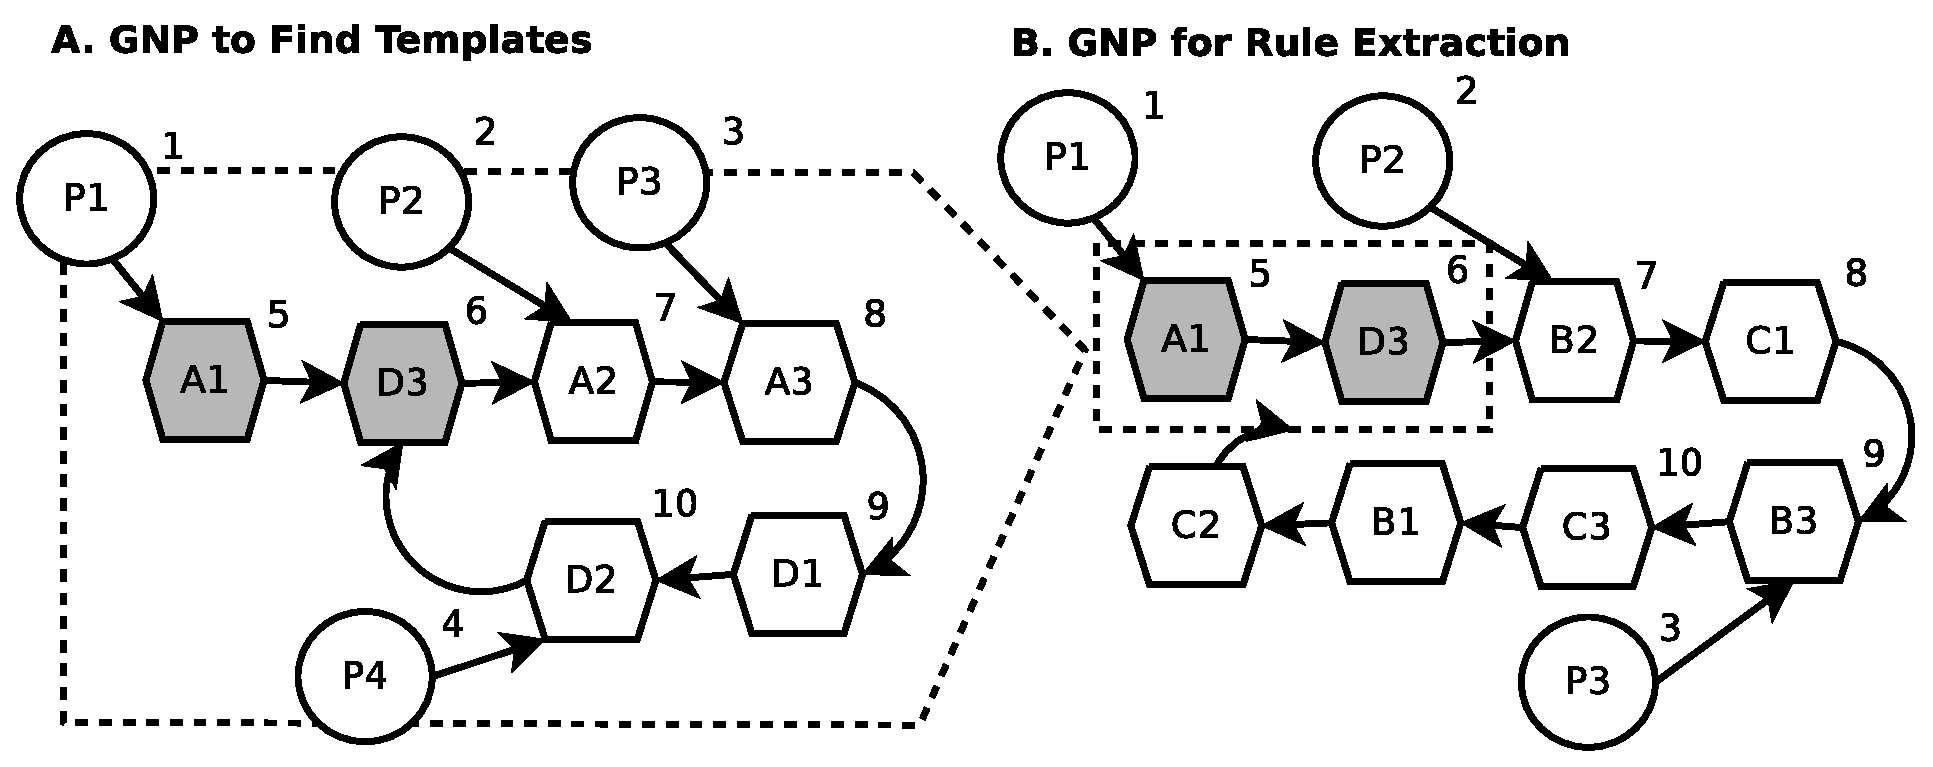
\includegraphics[width=14cm]{images/gnpdatamining2}
\caption{\label{newgnp} Node Arrangement Optimization in GNP}
\end{center}
\end{figure}

Table \ref{partial-random-combination-example2} shows a simple example of partial random for easy explanation. 
Each template contains attribute $A$ and $D$, and it is combined with the remaining attributes, that is $B$ and $C$. 
The generated rule of $A_{3} \wedge D_{3} \wedge B_{1} \wedge C_{2}$ obtains the highest score of rule (Eq. \ref{eq:fitness}) because it has long rule length and high coverage.

\begin{table}[tb]
\caption{\label{partial-random-combination-example2}Example of combination of templates with remaining attributes}
\begin{flushleft}
\begin{tabular}{|c|c|c|c|c|}
\hline 
Template & Remaining attributes & Coverage & Score of rule \tabularnewline
\hline 
$A_{2}\wedge D_{3}$ & $B_{1}\wedge C_{2}$ & 0 & 0\tabularnewline
\hline 
$A_{2}\wedge D_{3}$ & $B_{3}\wedge C_{2}$ & 10 & 40.4\tabularnewline
\hline 
$A_{1}\wedge D_{3}$ & $B_{3}$ & 24 & 34.5\tabularnewline
\hline 
$A_{3}\wedge D_{3}$ & $B_{1}\wedge C_{2}$ & 14 & 40.5\tabularnewline
\hline 
\end{tabular}
\end{flushleft}
\end{table}

\subsection{Rule Distribution with Knapsack Problem}
After all the records in a dataset are covered by rules extracted by GNP, KP is used to distribute rules to several sites. Rules with high coverage (elite) become the leaders of each site, 
then KP considers the similarity of the remaining rules to the leader rules (value) and coverage of the rules (weight) in order to distribute the remaining rules to the sites. Similarity of remaining rule $r_{1}$ to leader rule $r_{2}$ is calculated by Eq. \ref{eq:similarity}.

\begin{eqnarray}
\begin{array}{lll}
S(r_{1},r_{2})=\frac{N_{match}(r_{1},r_{2})}{Max\{N_{ante}(r_{1}),N_{ante}(r_{2})\}}
\end{array}
\label{eq:similarity}
\end{eqnarray}
$S(r_{1},r_{2})$ : similarity between rule $r_{1}$ and $r_{2}$, $N_{match}(r_{1},r_{2})$ : the number of matched attributes between $r_{1}$ and $r_{2}$, $N_{ante}(r)$ $(r\in\{r_{1},r_{2}\})$ : the number of attributes in rule $r$.

$Max\{N_{ante}(r_{1}),N_{ante}(r_{2})\}$ means that longer rule length becomes a divider to the number of matched attributes between two rules ($N_{match}(r_{1},r_{2})$). When the longer rule includes attributes that are not contained in the shorter rule, those attributes are assumed to be matched. Examples of similarity calculation are shown in Table \ref{remained-rules}. From Table \ref{remained-rules}, rule 2 shows the highest similarity to the leader. The leader rule does not have attribute $D$, so every attribute $D$ in the remaining rules is assumed to be matched.

\begin{table}
\caption{\label{remained-rules}Example of similarity calculation between leader and remaining rules}
\begin{flushleft}
\begin{tabular}{|c|c|c|c|c|c|c|}
\hline 
Rule & $A$ & $B$ & $C$ & $D$ & $N_{match}(r_{1},r_{2})$ & $S(r_{1},r_{2})$\tabularnewline
\hline 
Leader & $A_{1}$ & $B_{3}$ & $C_{2}$ & - & - & -\tabularnewline
\hline 
1 & *$A_{1}$ & $B_{2}$ & $C_{1}$ & *$D_{2}$ & 2 & 2/4\tabularnewline
\hline 
2 & $A_{2}$ & *$B_{3}$ & *$C_{2}$ & *$D_{1}$ & 3 & 3/4\tabularnewline
\hline 
3 & *$A_{1}$ & $B_{1}$ & *$C_{2}$ & - & 2 & 2/3\tabularnewline
\hline 
\end{tabular}
\end{flushleft}
* : matched attribute
\end{table}

\section{Simulations}
First, full random and partial random methods in the rule extraction of GNP are compared. Then, knapsack rule distribution is carried out and its results are compared with k-means and hierarchical clustering \cite{silhouette}.

\subsection{GNP Rule Extraction}

\begin{table*}[tb]
\caption{\label{gnp-rule-extraction-result-full}Results of GNP rule extraction
with full randomization in six datasets}


\begin{raggedright}
\begin{tabular}{|l|l|l|l|l|l|l|l|l|l|l|}
\hline 
\multirow{2}{*}{Attr} & \multicolumn{5}{c|}{Full Random} & \multicolumn{5}{c|}{Partial Random}\tabularnewline
\cline{2-11} 
 & Itr  & $n$  & Rule  & Cvrg  & Score  & Itr  & $n$  & Rule  & Cvrg  & Score\tabularnewline
\hline 
3  & 34  & 2.33  & 34  & 29  & 10.15  & 25  & 3.00  & 39  & 23  & 20.29\tabularnewline
\hline 
3  & 78  & 2.23  & 12  & 808  & 10.01  & 45  & 3.00  & 18  & 526  & 20.02\tabularnewline
\hline 
8  & 564  & 3.45  & 23  & 42  & 20.23  & 435  & 6.62  & 43  & 22  & 50.26\tabularnewline
\hline 
8  & 1056  & 2.76  & 52  & 182  & 10.07  & 786  & 5.43  & 57  & 145  & 40.13\tabularnewline
\hline 
15  & 6290  & 2.46  & 34  & 20  & 10.15  & 5987  & 7.35  & 45  & 21  & 60.23\tabularnewline
\hline 
15  & 987  & 4.23  & 12  & 833  & 30.02  & 789  & 11.25  & 8  & 1110  & 100.03\tabularnewline
\hline 
\multicolumn{5}{|l|}{} & 90.63  & \multicolumn{4}{l|}{} & 290.96\tabularnewline
\hline 
\end{tabular}
\par\end{raggedright}

Attr : the number of attributes, Itr : number of iterations to cover all the records, \\ $n$ : mean length of each rule, Rule : the average number of rules, \\
Cvrg : mean coverage, Score : mean score of rules 
\end{table*}

The result comparison between two node arrangement methods, that is, full randomization and partial randomization, is shown in Table \ref{gnp-rule-extraction-result-full}. Six datasets are used for the comparison, where the number of data (5000) and the data variation (50\%) are the same, however the number of attributes is different. The performance evaluation is executed to compare the iterations needed to cover all the data, 
the mean rule length,
the number of extracted rules, 
and the mean score of rules.
Here, iteration means the number of individuals created in the rule extraction until all the records are covered.

When the number of attributes is increased, the number of iterations needed to cover all the data tends to be increased. However, comparing the iteration needed by full randomization and partial randomization, partial randomization shows better results, i.e., less iteration are needed. Rules are extracted until all the records in the dataset are covered, but the records that have been already covered will not be re-included. Significant difference between full random and partial random is in the average node length where partial random basically shows longer length. By finding frequent item-set (template), partial random can establish the minimum node length of rules in each cluster. Partial random basically extracts larger number of longer rules than full random, therefore, the mean scores of rules extracted by partial random shows better results.
From the next section, partial random method is used in the simulations.

\subsection{Knapsack Rule Distribution}
Here, silhouette value \cite{silhouette1} is used to evaluate the clustering results. Silhouette provides a succinct graphical representation of how well each object lies within its cluster. Silhouette value is calculated by Eq. \ref{eq:silhouette}.

\begin{eqnarray}
\begin{array}{lll}
s = \frac{b - a}{\max\{a,b\}} \\
\quad= \begin{cases} 1-a/b, & \mbox{if } a < b \\ 0, & \mbox{if } a = b \\ b/a-1, & \mbox{if } a > b \\ \end{cases} 
\end{array}
\label{eq:silhouette}
\end{eqnarray}
\begin{description}
\item [s:] Silhouette value for a single sample. The Silhouette value for a set of samples is given as the mean of the Silhouette values of each sample.
\item [a:] mean distance between a sample and all other points in the same cluster.
\item [b:] mean distance between a sample and all other points in the second nearest cluster.
\end{description}

The results of rule distribution are shown in Table \ref{knapsack-result}. All the simulations are executed with the same number data (5000) and data variation (50\%).
$k$ is the number of clusters (sites),
``Balance of clusters capacity" shows the proportion of capacity of each site, for example, 1:1:1:1 means all the four sites have the same size, and 1:4:2:1 means the second site (size four) is four times larger than the first site (size one).
``Average, Max and Min" show the data on Silhouette values obtained by the generated clusters. According to the silhouette values, the proposed method shows good clustering ability in the case of larger $k$ and the balanced cluster capacity. The silhouette values are decreased as $k$ decreases and the cluster capacity is unbalanced. This situation happens because of the capacity incompatibility between rule coverage and cluster capacity. For example, when the cluster capacity is only 100 data left, and the coverage of a certain rule is 120 data, 20 data will be distributed to another cluster, which affects the silhouette result. If the number of sites $k$ is larger, various kinds of rules can be distributed to many sites, then more closer (similar) rules can be included in each cluster, which contributes to better silhouette values.    
If the cluster capacity is unbalanced, some sites have larger capacity and some have smaller. The sites with larger capacity have to contain various kinds of rules (which sometimes have a little far distance from each other), therefore, the silhouette values become smaller.  

\begin{table}[tb]
\caption{\label{knapsack-result}Result of Knapsack Problem (Silhouette values)}
\begin{tabular}{|l|l|l|l|l|}
\hline 
$k$ & Balance of Cluster Capacity & Average & Max & Min\tabularnewline
\hline 
8 & 1:1:1:1:1:1:1:1 & 0.97 & 0.98 & 0.92\tabularnewline
\hline 
8 & 4:2:4:6:4:2:7:5 & 0.91 & 0.97 & 0.88\tabularnewline
\hline 
6 & 1:1:1:1:1:1 & 0.87 & 0.91 & 0.86\tabularnewline
\hline 
6 & 1:5:2:6:3:2 & 0.82 & 0.88 & 0.78\tabularnewline
\hline 
4 & 1:1:1:1 & 0.75 & 0.81 & 0.70\tabularnewline
\hline 
4 & 1:4:2:1 & 0.72 & 0.79 & 0.68\tabularnewline
\hline 
\end{tabular}
\end{table}

\subsection{Comparison with K-means and Hierarchical Clustering}
Clustering methods used for the comparison are k-means and hierarchical clustering \cite{silhouette} because both methods also use distance measure. k-means is based on a centroid concept for cluster separation and the centroids also represent each cluster. Hierarchical clustering is selected for the comparison because it uses the similar concept to the proposed method using leader rules to distribute rules.
Although both methods can set the number of clusters to be created, they do not have a function to measure cluster capacity as KP. Thus, the cluster capacity problem is not discussed in this comparison.
The proposed method can execute clustering considering the cluster capacities, which is one of the advantages over k-means and hierarchical clustering.



\begin{table}[tb]
\vspace{1em}
\caption{\label{dataset-used-to-comparison}Value ranges of attributes in the dataset}
\begin{flushleft}
\begin{tabular}{|l|l|l|l|}
\hline 
Attribute & Min Value & Max Value\tabularnewline
\hline 
A & 100 & 500\tabularnewline
\hline 
B & 1000 & 2000\tabularnewline
\hline 
C & 700 & 1500\tabularnewline
\hline 
D & 1 & 5\tabularnewline
\hline 
E & 15 & 95\tabularnewline
\hline 
F & 10000 & 30000\tabularnewline
\hline 
G & 5000 & 50000\tabularnewline
\hline 
H & 1 & 10\tabularnewline
\hline 
\end{tabular}
\par\end{flushleft}
\end{table}

\begin{table}[tb]
\caption{Data on Silhouette values in the eight cases}
\label{silhouette-comparison}
\begin{flushleft}
\begin{tabular}{|l|l|l|l|l|l|l|}
\hline 
case & $k$ & Attribute & Data Amount & GNP-KP & K-means & Hierarchical \tabularnewline
\hline 
1 & 10 & 4 & 1000 & 0.921 & 0.912 & 0.852 \tabularnewline
\hline 
2 & 10 & 4 & 2000 & 0.902 & 0.899 & 0.831 \tabularnewline
\hline 
3 & 8 & 6 & 3000 & 0.843 & 0.832 & 0.780 \tabularnewline
\hline 
4 & 8 & 6 & 4000 & 0.823 & 0.801 & 0.648 \tabularnewline
\hline 
5 & 6 & 8 & 5000 & 0.576 & 0.356 & 0.521 \tabularnewline
\hline 
6 & 6 & 8 & 6000 & 0.532 & 0.322 & 0.501 \tabularnewline
\hline 
7 & 4 & 10 & 7000 & 0.325 & 0.104 & 0.312 \tabularnewline
\hline 
8 & 4 & 10 & 8000 & 0.312 & 0.092 & 0.303 \tabularnewline
\hline 
\end{tabular}


$k$ : the number of clusters,
Attribute : the number of attributes
%Variation : variation of dataset[\%]
\end{flushleft}
\end{table}

\begin{figure}
\begin{center}
\includegraphics[width=12cm]{images/silhouette}
\caption{\label{silhouette} Comparison of silhouette values in eight cases}
\end{center}
\end{figure}

\begin{figure}
\begin{center}
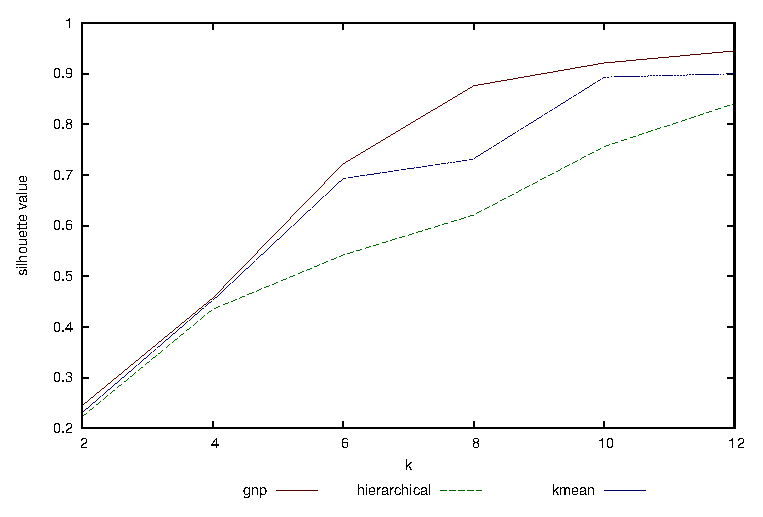
\includegraphics[width=12cm]{images/silhouette-k}
\caption{\label{silhouette-k} Comparison of silhouette values for various $k$}
\end{center}
\end{figure}

\begin{figure}
\begin{center}
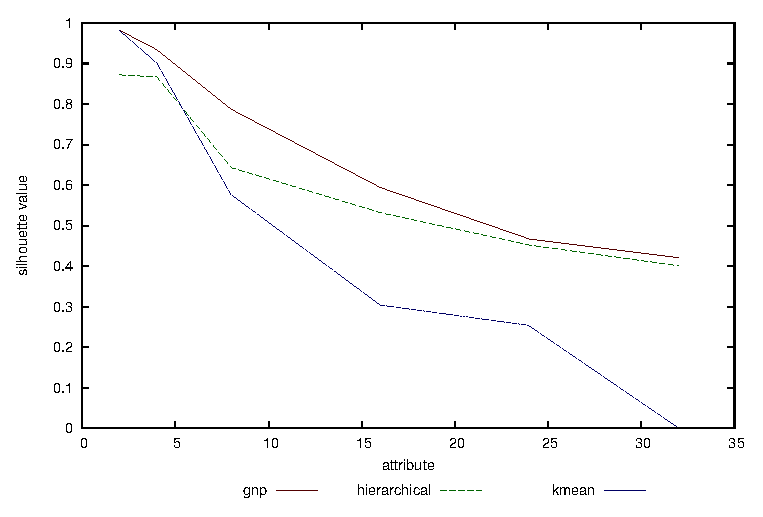
\includegraphics[width=12cm]{images/silhouette-attribute}
\caption{\label{silhouette-attribute} Comparison of silhouette values for various number of attribute}
\end{center}
\end{figure}

The features of attributes contained in the dataset for the comparison is shown in Table \ref{dataset-used-to-comparison}. 
In this simulation, eight datasets are prepared, where the values of each record are determined randomly in the ranges of each attribute and the data variation is fixed at 50\%, however the number of records in each case is different.
Table \ref{silhouette-comparison} shows more information on the eight datasets and Silhouette values obtained by the proposed method (GNP-KP), k-means and hierarchical clustering (HC). 
Fig. \ref{silhouette} graphically shows the silhouette values obtained by each method in the eight cases. When the number of attributes is small, the values obtained by GNP-KP and k-means are almost the same and higher than HC, however as the number of attributes increases, k-means shows lower values and HC shows higher values than k-means. GNP-KP shows the highest values in all the cases.

Fig. \ref{silhouette-k} shows the relation between silhouette values and $k$ in the dataset with four attributes and 5000 data. As $k$ increases, silhouette values of the three methods increase, where GNP-KP shows better results in every case. Fig. \ref{silhouette-attribute} shows the relation between silhouette values and the number of attributes in the dataset with $k=4$ and 5000 data. It can be seen from Fig. \ref{silhouette-attribute} that k-means is good to process datasets with the small number of attributes, but the silhouette values are decreased significantly as the number of attributes increases. HC shows relatively stable results for the changes of the number of attributes but does not reach the highest results. GNP-KP shows the decrease of silhouette values, but still makes better results in the six cases.

\begin{table*}[tb]
\caption{\label{extracted-nodes-and-its-coverage}Generated value ranges of nodes and their coverage}
\begin{flushleft}
\begin{tabular}{|l|l|l|l|l|l|l|}
\hline 
\multirow{1}{*}{Attr} & Ranges & Cvrg & Ranges & Cvrg & Ranges & Cvrg\tabularnewline
\hline 
\multirow{2}{*}{A} & {[}140,173{]} & 225 & {[}221,238{]} & 377 & {[}270,317{]} & 128\tabularnewline
\cline{2-7} 
 & {[}339,500{]} & 270 & \multicolumn{4}{l|}{}\tabularnewline
\hline 
\multirow{2}{*}{B} & {[}1063,1146{]} & 164 & {[}1215,1251{]} & 213 & {[}1310,1316{]} & 115\tabularnewline
\cline{2-7} 
 & {[}1368,1394{]} & 238 & {[}1397,1406{]} & 100 & {[}1414,2000{]} & 170\tabularnewline
\hline 
\multirow{3}{*}{C} & {[}744,787{]} & 52 & {[}798,829{]} & 180 & {[}873,890{]} & 206\tabularnewline
\cline{2-7} 
 & {[}930,938{]} & 257 & {[}962,981{]} & 74 & {[}1022,1022{]} & 57\tabularnewline
\cline{2-7} 
 & {[}1055,1104{]} & 37 & {[}1133,1500{]} & 137 & \multicolumn{2}{l|}{}\tabularnewline
\hline 
D & {[}1,2{]} & 398 & {[}3,5{]} & 602 & \multicolumn{2}{l|}{}\tabularnewline
\hline 
E & {[}21,26{]} & 97 & {[}29,33{]} & 267 & {[}37,95{]} & 636\tabularnewline
\hline 
\multirow{3}{*}{F} & {[}11045,11319{]} & 308 & {[}12329,13300{]} & 189 & {[}14394,14847{]} & 162\tabularnewline
\cline{2-7} 
 & {[}14891,15502{]} & 72 & {[}16495,16879{]} & 72 & {[}18109,18152{]} & 93\tabularnewline
\cline{2-7} 
 & {[}18913,20096{]} & 34 & {[}21084,30000{]} & 70 & \multicolumn{2}{l|}{}\tabularnewline
\hline 
\multirow{4}{*}{G} & {[}5858,6890{]} & 166 & {[}8277,9055{]} & 345 & {[}10787,12407{]} & 151\tabularnewline
\cline{2-7} 
 & {[}13629,13832{]} & 34 & {[}15876,17152{]} & 33 & {[}17960,18525{]} & 122\tabularnewline
\cline{2-7} 
 & {[}19876,20841{]} & 54 & {[}22367,23533{]} & 41 & {[}23794,25908{]} & 26\tabularnewline
\cline{2-7} 
 & {[}27327,50000{]} & 28 & \multicolumn{4}{l|}{}\tabularnewline
\hline 
H & {[}1,1{]} & 446 & {[}2,3{]} & 113 & {[}4,10{]} & 441\tabularnewline
\hline 
\end{tabular}
\\ Attr : Attribute, Cvrg : Coverage
\end{flushleft}
\end{table*}

\begin{table*}[tb]
\caption{\label{nodes-substances-on-each-sites}Node substances in each site}
\begin{flushleft}
\begin{tabular}{|c|l|c|c|}
\hline 
Site & Attributes & Capacity & Data\tabularnewline
\hline 
1 & $\{A3,B5,C5,D2,E2,F7,G2,H1\}$ & 100 & 84\tabularnewline
\hline 
2 & $\{A1,A3,B1,B5,C4,D2,E3,F2,F5,G1,G2,H1\}$ & 500 & 295\tabularnewline
\hline 
3 & $\{A4,B6,C8,D2,E3,F3,G2,G3,H1\}$ & 200 & 68\tabularnewline
\hline 
4 & $\{A2,B2,B4,C1,C2,C5,D2,E2,F1,$ & 600 & 420\tabularnewline
 & $F4,F8,G3,G5,G6,G8,H3\}$ &  & \tabularnewline
\hline 
5 & $\{A1,C3,D1,E1,F6,G7,G9,H1,H2\}$ & 300 & 120\tabularnewline
\hline 
6 & $\{A4,B2,C6,D1,E3,F1,G4,H3\}$ & 200 & 163\tabularnewline
\hline 
\end{tabular}
\end{flushleft}
\end{table*}

The results of the clustering executed by GNP-KP are analyzed using Table \ref{extracted-nodes-and-its-coverage} and \ref{nodes-substances-on-each-sites} in detail. Table \ref{extracted-nodes-and-its-coverage} shows the value ranges of the generated nodes for each attribute and their coverage. The different number of nodes are generated for each attribute depending on their value ranges as shown in Table. \ref{dataset-used-to-comparison}. For example, attribute $D$ just has two nodes because its value range is only between one and five, but attribute $G$ has ten nodes because it has a wider value range which is between 5000 and 50000. Each attribute also shows unbalanced coverage for each range. For example, one of the nodes of attribute $F$ dominates the data with the range between 11045 and 11319 which shows larger coverage compared to other nodes. This domination has an effects on the nodes contained in each site (cluster), which is shown in Table \ref{nodes-substances-on-each-sites}. Sites with larger capacity contain rules with various kinds of attributes and more than one variation of node for each attribute. For example, in site 4, there are ${B2,B4}$ for attribute $B$ and ${C1,C2,C5}$ for attribute $C$. This result indicates site 4 contains some rules with the same attributes of different value ranges; for example, $A2\wedge B2\wedge C1\wedge E2\wedge F1\wedge G3\wedge H3$ and $A2\wedge B4\wedge C2\wedge D2\wedge F1\wedge G3\wedge H3$. Sites with larger capacity have higher probability to contain more variation of records.

As described in section \ref{sec:partial-random} on partial randomization, a combination of attributes (nodes) with high coverage would also result in high coverage. However, because each site (cluster) has a limit of capacity, attributes with high coverage would become substances of several sites. Since many data having major characteristics are difficult to be put into one site due to the limit of its site capacity, such data will be distributed to several sites. This problem could be solved by reducing the ranges of attributes, which contributes to decreasing the range domination. However, it will increase the calculation cost and influence the processing time.

\section{Conclusions}
This paper proposes a novel clustering method combining Genetic Network Programming and Knapsack Problem to handle record clustering. The proposed method can find  good combinations of attributes to create rules for clustering, and also consider the capacity of sites to distribute rules. From the simulation results, the proposed method shows better clustering ability than k-means and hierarchical clustering in the eight kinds of datasets. In the future, we will consider the replication problems of distributed databases, where the query frequency is considered in the clustering problems and frequently accessed data will be stored in several sites to decrease the load of the accesses.



\bibliographystyle{apacitex}
\bibliography{IEEEabrv,references}


\end{document}